 \documentclass{beamer}
\usetheme{Berlin}
\usecolortheme{beaver}
\usepackage[ngerman]{babel}
\usepackage{graphicx}
\usepackage[utf8]{inputenc}
\usepackage{times}
\usepackage[T1]{fontenc}
\usepackage{subfigure}
\usepackage{moreverb}

\title{Classifying Colon Cancer Colonoscopy Images Using Edge Histograms}
\author[]{Samy Dafir \\Dominik Baumgartner \\Sebastian Strumegger}
\date{\today}
\begin{document}
\frame{\titlepage}

\begin{frame}
    \frametitle{Content} 
    \tableofcontents 
\end{frame}

\section{Task - Overview}
\begin{frame}
	\frametitle{Task - Overview}
    \begin{block}{What?}
	    \begin{itemize}
		    \item Colon cancer colonoscopy images
		    \item Edge histograms
            \item KNN: K Nearest Neighbors - Classification
	    \end{itemize}
    \end{block}
\end{frame}

\begin{frame}
	\frametitle{Task - Overview}
    \begin{block}{How?}
	    \begin{enumerate}
		    \item Preprocess images
		    \item Perform edge detection
		    \item Extract features (e.g. edge lengths)
            \item Compute Edge Histogram
            \item Classify with KNN
            \item Analyze the results
	    \end{enumerate}
    \end{block}
\end{frame}

\section{Edge Detection}

\begin{frame}
	\frametitle{Overview}
	\begin{itemize}
		\item What are Edges
		\item Edge Detection
		\item First Derivative
		\item Second Derivative
		\item Canny Edge Detection
	\end{itemize}
\end{frame}
\begin{frame}
		\begin{block}{Edges:}
			Edges are pixels, in which the image intensity function changes its
			magnitude
		\end{block}
	\begin{figure} 
		\subfigure[Original Image]{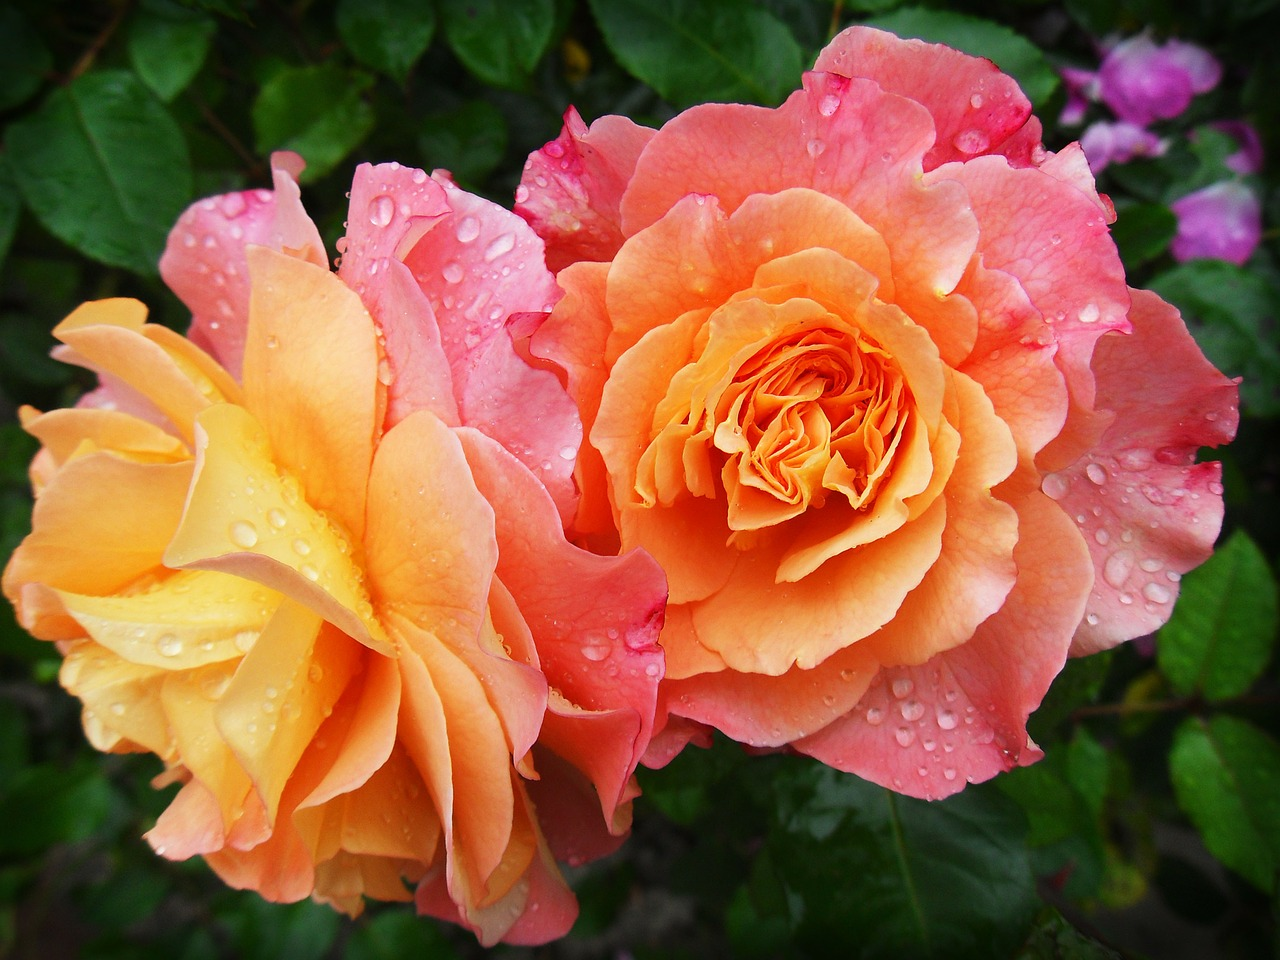
\includegraphics[width=0.49\textwidth]{edge1.jpg}} 
		\subfigure[Image after Edge Detection]{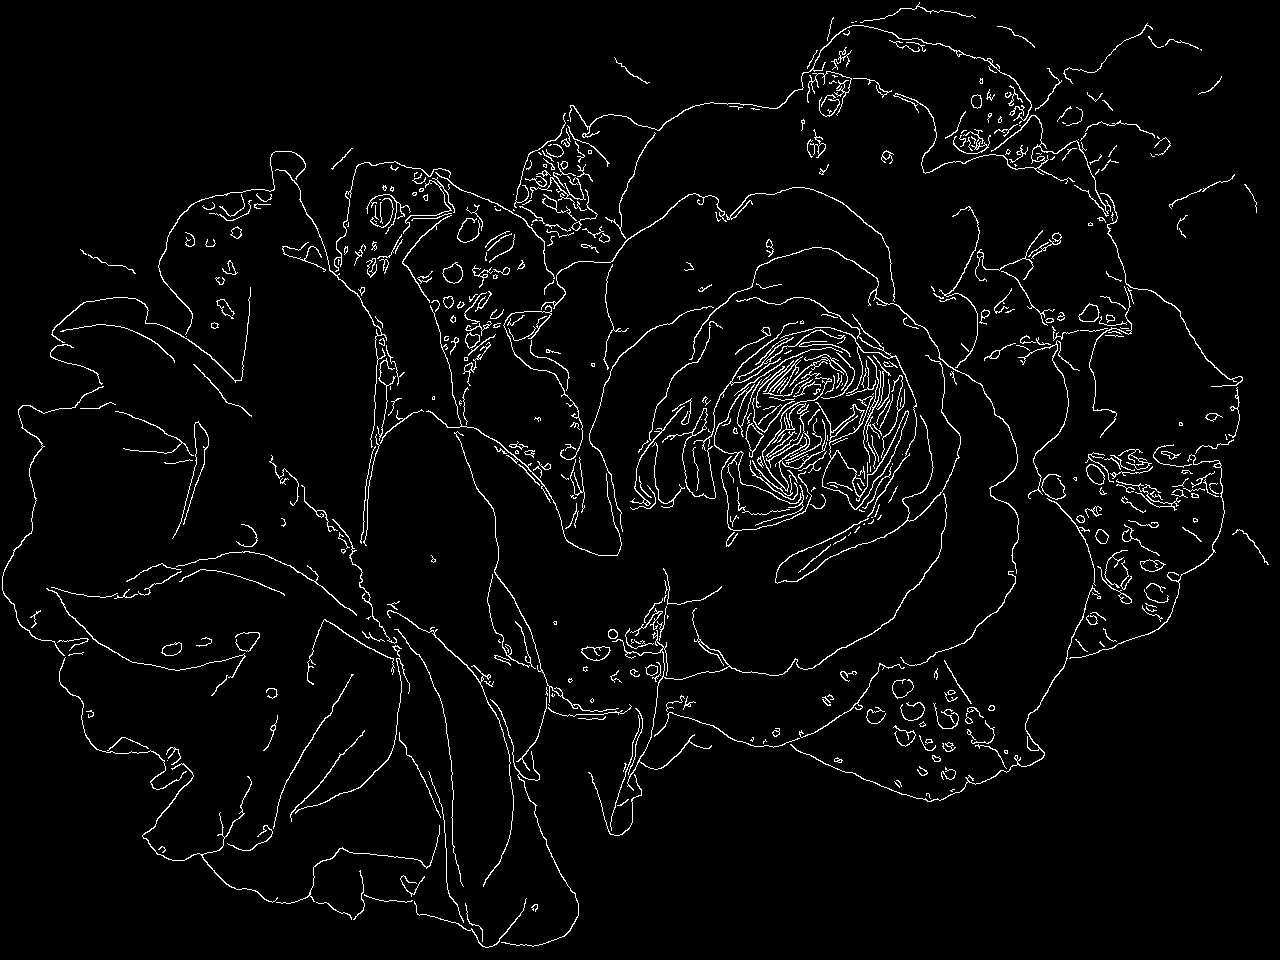
\includegraphics[width=0.49\textwidth]{edge2.jpg}} 
		\caption{Edge Detection using Canny} 
		\end{figure}
\end{frame}

\begin{frame}
	\begin{block}{Edge Detection:}
		Almost every Edge Detector uses either the first derivative or the second derivative of the intensity function. 
	\end{block}
	\begin{figure} 
		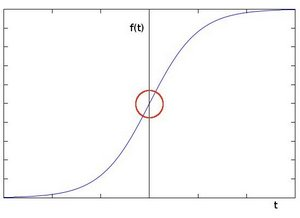
\includegraphics[width=0.49\textwidth]{edge3.jpg}
		\caption{Intensity function} 
	\end{figure}
\end{frame}

\begin{frame}
	\begin{block}{First Derivative:}
		Sobel-, Roberts-, Robinson-, Kirsch-Operator 
	\end{block}
	\begin{figure} 
		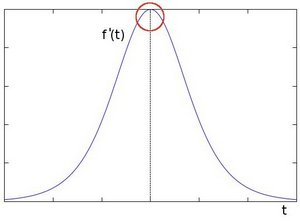
\includegraphics[width=0.49\textwidth]{edge4.jpg}
		\caption{Intensity function - First derivative} 
	\end{figure}
\end{frame}

\begin{frame}
	\begin{block}{Second Derivative:}
	Laplace-, Mexican-Hat-Operator 
	\end{block}
	\begin{figure} 
		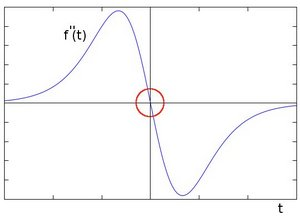
\includegraphics[width=0.49\textwidth]{edge5.jpg}
		\caption{Intensity function - Second derivative} 
	\end{figure}
\end{frame}

\begin{frame}
	\begin{block}{Canny Edge Detection:}
		\begin{itemize}
			\item Low error rate
			\item Good localization
			\item Minimal response
		\end{itemize}
	\end{block}
\end{frame}

\begin{frame}
	\begin{block}{Steps:}
		\begin{enumerate}
			\item Filter out noise using Gaussian filter
			\item Find the intensity gradient using Sobel-Operator\\
			$G = \sqrt{G_x^2 + G_y^2}$ or  $G = |G_x| + |G_y|$
			\item Non-maximum suppression
			\item Hysteresis
		\end{enumerate}
	\end{block}
\end{frame}


\section{Implementation}

\begin{frame}
	\frametitle{Overview}
	\begin{itemize}
		\item Development and Frameworks
		\item Image Enhancement
		\item Edge Detection
		\item Histograms
		\item Edge Lengths
		\item Edge Orientation
		\item Image Classification
	\end{itemize}
\end{frame}


\begin{frame}
	\frametitle{Development and Frameworks}
	Developed using:
	\begin{itemize}
		\item Java 8
		\item OpenCV for Java
		\item Eclipse Neon
	\end{itemize}
	
\end{frame}

\begin{frame}
	\frametitle{Image Enhancement and Conversion}
	\begin{block}{}
		\begin{itemize}
			\item Color Space Conversion
			\item Normalization
			\item CLAHE
			\item All part of OpenCV
		\end{itemize}
	\end{block}
	
\end{frame}

\begin{frame}[fragile]
	\frametitle{Image Enhancement and Conversion}
	\textbf{RGB to HSV}
	\\
	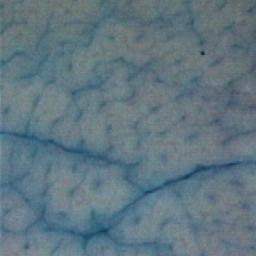
\includegraphics[width = 4cm]{before_3.png}
	\raisebox{0.75\height}{
\includegraphics[width = 1.5cm]{arrow_right.png}}
	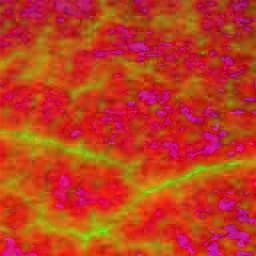
\includegraphics[width = 4cm]{after_3.jpg}
	\begin{verbatimtab}
Imgproc.cvtColor(matrix, matrix, colorSpace)
colorSpace: e.g. Imgproc.COLOR_RGB2HSV
	\end{verbatimtab}
\end{frame}

\begin{frame}[fragile]
	\frametitle{Image Enhancement and Conversion}
	Normalization:
	\begin{verbatimtab}
Core.normalize(matrix,matrix,255,0,
 Core.NORM_MINMAX);
	\end{verbatimtab}
	
	CLAHE: 
	\begin{verbatimtab}
Mat channel = new Mat();
Core.extractChannel(matrix, channel, i);
CLAHE clahe = Imgproc.createCLAHE();
clahe.apply(channel, channel);
Core.insertChannel(channel, matrix, i);
	\end{verbatimtab}
\end{frame}

\begin{frame}
	\frametitle{Image Enhancement and Conversion}
	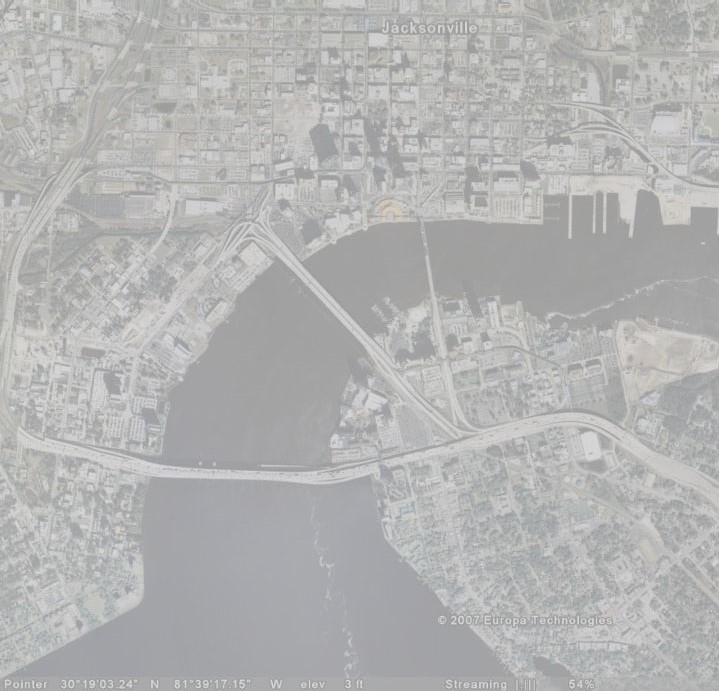
\includegraphics[width = 4.6cm]{before.jpg}
	\raisebox{0.9\height}{
\includegraphics[width = 1.5cm]{arrow_right.png}}
	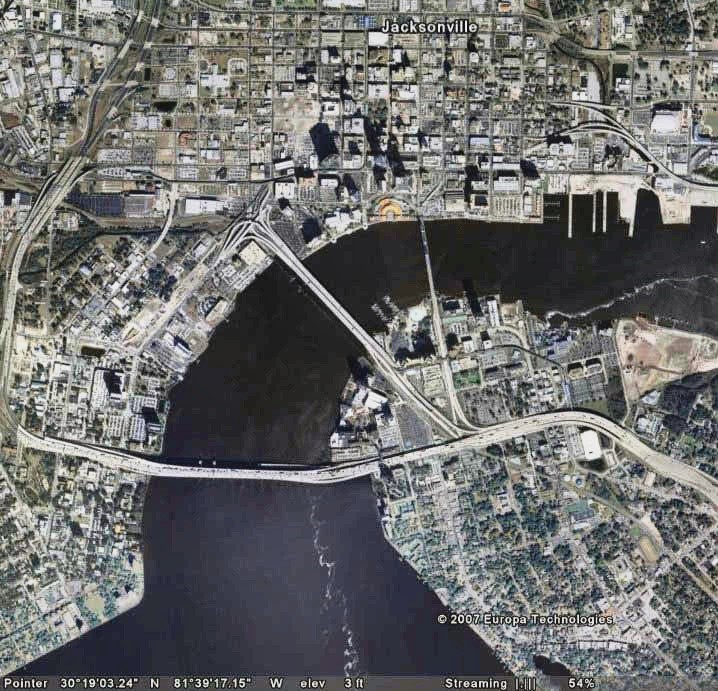
\includegraphics[width = 4.6cm]{after.jpg}
\end{frame}

\begin{frame}
	\frametitle{Image Enhancement and Conversion}
	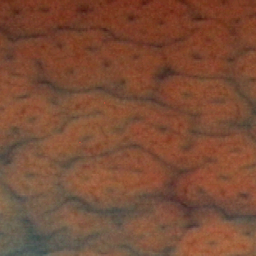
\includegraphics[width = 4cm]{before_1.png}
	\raisebox{0.75\height}{
\includegraphics[width = 1.5cm]{arrow_right.png}}
	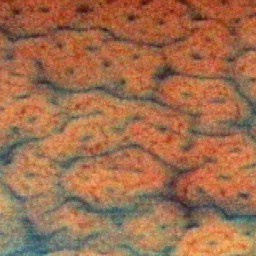
\includegraphics[width = 4cm]{after_1.jpg}
\end{frame}

\begin{frame}
	\frametitle{Edge Detection}
	\begin{block}{}
		\begin{itemize}
			\item Grayscale Conversion
			\item Canny Edge Detector
		\end{itemize}
	\end{block}
\end{frame}

\begin{frame}[fragile]
	\frametitle{Edge Detection}
	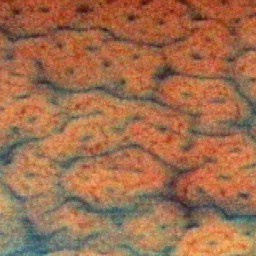
\includegraphics[width = 4cm]{after_1.jpg}
	\raisebox{0.75\height}{
\includegraphics[width = 1.5cm]{arrow_right.png}}
	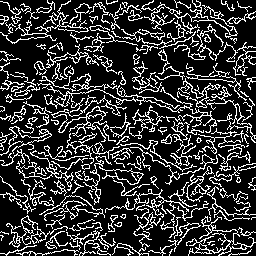
\includegraphics[width = 4cm]{edges_detected.png}		
	\begin{verbatimtab}
Imgproc.Canny(matrix, matrix, 
 lowThresh, highThresh);
	\end{verbatimtab}
\end{frame}

\begin{frame}
	\frametitle{Edge Histograms}
	\begin{block}{Definition}
		\begin{itemize}
			\item Characteristics of an image e.g. edge lengths
			\item Partition characteristic attributes into bins
			\item In our case: Edge lengths \& orientations
			\item Length: Image has\\
			5 edges of length 0 - 20 pixels\\
			20 edges of length 100 - 120 pixels
		\end{itemize}
	\end{block}
	
\end{frame}

\begin{frame}
	\frametitle{Edge Histograms}
	Simple Example:\\
	10.0, 20.0, 23.0, 30.0, 28.0, 18.0, 1\\
	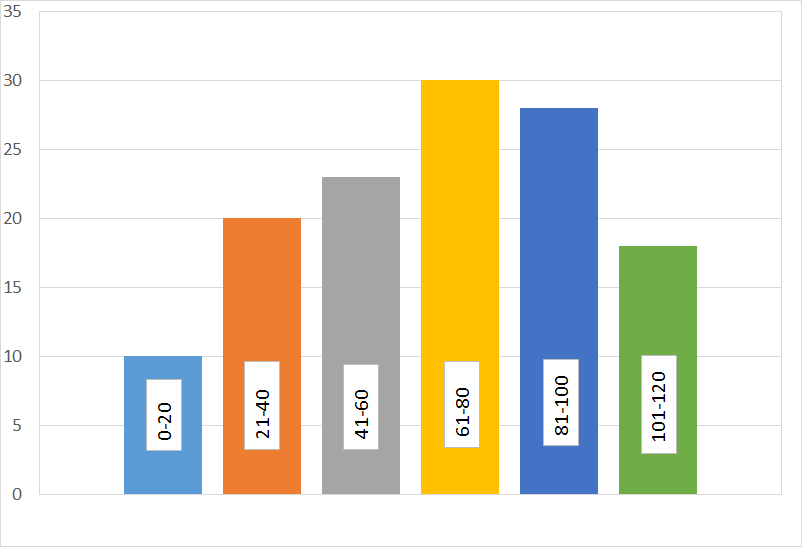
\includegraphics[width = 8cm]{histogram.png}	
	
\end{frame}

\begin{frame}[fragile]
	\frametitle{Edge Histograms}
	\begin{itemize}
		\item Histogram data for each example image collected in a hist-file.
		\item Specify Category. Here: Cancer stage
		\item Example:\\
		\begin{verbatimtab}[1]
210.0,3.0,170.0,142.0,126.0,93.0,32.0,16.0,1
192.0,2.0,181.0,139.0,119.0,87.0,32.0,17.0,1
143.0,1.0,172.0,147.0,128.0,91.0,30.0,16.0,1
		\end{verbatimtab}
		
	\end{itemize}
	
\end{frame}

\begin{frame}
	\frametitle{Edge Lengths}
	\begin{block}{Prequisites}
		\begin{itemize}
			\item Image with detected Edges
			\item Edges white
			\item Rest black
			\item Not entirely given $\rightarrow$ Threshold set at grayscale 200
		\end{itemize}
	\end{block}
	
\end{frame}

\begin{frame}
	\frametitle{Edge Lengths}
	\begin{block}{Algorithm}
		Iterate over all pixels
		\begin{enumerate}
			\item Check if pixel is white $\rightarrow$ new edge found
			\item Check immediate neighbours: if white $\rightarrow$ add pixel to edge
			\item Follow white path until no more connected white pixels
			\item Add all passes pixels to Collection of used pixels
			\item Add one to category with detected length
			\item Continue iterating and start at 1
			
		\end{enumerate}
	\end{block}
\end{frame}


\begin{frame}[fragile]
	\frametitle{Edge Lengths}
	\begin{block}{Algorithm}
		\begin{verbatimtab}[4]
function measureEdge(pixel) {
	length = 1
	for each surrounding pixel p:
		if p == white
			length += measureEdge(p)
	
	return length
}
		\end{verbatimtab}
	\end{block}
\end{frame}

\begin{frame}
	\frametitle{Edge Orientation}
	\begin{itemize}
		\item Requires edge detected image
		\item Use sobel operator to detect edges
		\item Extract edge orientations from image (OpenCV)
		\item Partition edges into bins
		\item Bin content: pixels part of edge with certain orientation
		\item Category: range of angles
	\end{itemize}
	
	
\end{frame}

\begin{frame}
	\frametitle{Image Classification}
	\begin{enumerate}
		\item Classify all example images $\rightarrow$ create file with histograms
		\item Create List of Feature Vectors
		\item Enhance image to classify
		\item Create Feature Vector
		\item KNN: Compare new vector all vectors in list\\
		$\rightarrow$ euclidean distance\\
		\item Select K vectors with smallest distance
		\item Classification: category found most often
	\end{enumerate}
	
\end{frame}

\begin{frame}
	\frametitle{Paramter Optimization}
	\begin{block}{}
	Difference between a good and \\barely functional program 
	\end{block}
	\begin{itemize}
		\item Selection of input images
		\item Thresholds for edge detection
		\item Edge Lengths: number of bins, range of lengths in bins
		\item Weights of features:  all equally significant
		\\Lengths: per edge
		\\Orientation: per pixel
		
	\end{itemize}
	
\end{frame}

\section{Problems}
\begin{frame}
	\frametitle{Problems}
    \begin{block}{Encountered Problems}
	    \begin{itemize}
		    \item Fine tuning of parameters
	    \end{itemize}
    \end{block}
\end{frame}

\section{Results}
\begin{frame}
	\frametitle{Results}
    \begin{block}{Colormodels compared}
    	\begin{itemize}
    		\item enhanced RGB
    		\item HSV
    		\item Twice enhanced RGB
    	\end{itemize}
    \end{block}
\end{frame}

\begin{frame}
	\frametitle{Results}
    \begin{block}{Edgelength vs Edge Orientation vs both}
    \end{block}
\end{frame}

\end{document}
